\documentclass{tufte-handout}

\usepackage{style}

\begin{document}

\tma{04} % TMA number

\section{Part B}

%Question 9
Question 9 from section B
\begin{question}

\[ B_{d}((0,0),1), B_{d}[(0,0),1], \text{ and } S_{s}((0,0),1)   \]

By \textup{Defintion 2.6 HB Chapter 14 p 72}

\qpart

The open ball on metric 
\[ d((a_{1},a_{2}),(b_{1},b_{2})) = 6|b_{1} - a_{1} + |b_{2} - a_{2} \]

is given by
\begin{align*}
B_{d}((0,0),1) &= \{ (x,y) \in \R^{2} : d((x,y),(0,0)) < 1 \} \\[8pt]
&= \{ (x,y) \in \R^{2} : 6|x - 0| + |y - 0| < 1 \} \\[8pt]
&= \{ (x,y) \in \R^{2} : 6|x| + |y| < 1 \}      
\end{align*}

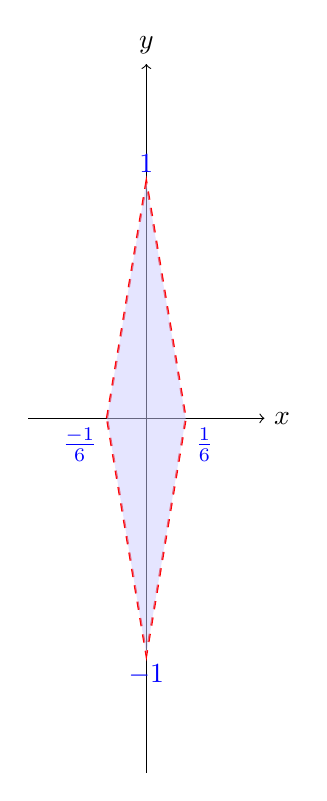
\begin{tikzpicture}[scale=3]
    %axis
    \draw[->] (-0.5,0) -- (0.5,0) node[right] {$x$};
    \draw[->] (0,-1.5) -- (0,1.5) node[above] {$y$};

    %boundry (dashes)
    \draw[thick, dashed, red] (-1/6,0) -- (0,1) -- (1/6,0) -- (0,-1) -- cycle;
    \fill[blue!20,opacity=0.5] (-1/6,0) -- (0,1) -- (1/6,0) -- (0,-1) -- cycle;

    %labels
    \node[blue, below left] at (-1/6,0) {$\frac{-1}{6}$};
    \node[blue, below right] at (1/6,0) {$\frac{1}{6}$};
    \node[blue, above] at (0,1) {$1$};
    \node[blue, below] at (0,-1) {$-1$};
\end{tikzpicture}

The closed ball on metric
\[ d((a_{1},a_{2}),(b_{1},b_{2})) = 6|b_{1} - a_{1} + |b_{2} - a_{2} \]

is given by
\begin{align*}
B_{d}[(0,0),1] &= \{ (x,y) \in \R^{2} : d((x,y),(0,0)) \leq 1 \} \\[8pt]
&= \{ (x,y) \in \R^{2} : 6|x - 0| + |y - 0| \leq 1 \} \\[8pt]
&= \{ (x,y) \in \R^{2} : 6|x| + |y| \leq 1 \}      
\end{align*}

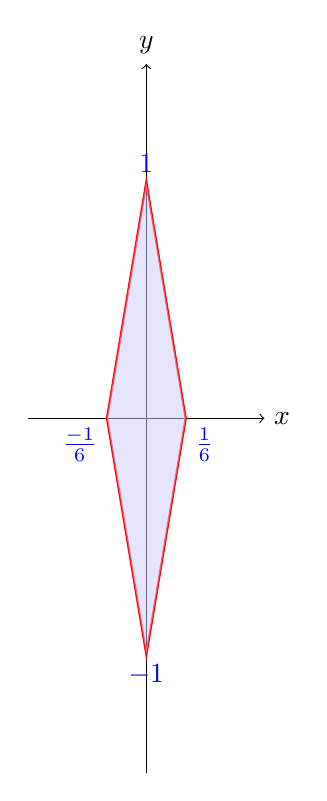
\begin{tikzpicture}[scale=3]
    %axis
    \draw[->] (-0.5,0) -- (0.5,0) node[right] {$x$};
    \draw[->] (0,-1.5) -- (0,1.5) node[above] {$y$};

    %boundry (solid)
    \draw[thick, red] (-1/6,0) -- (0,1) -- (1/6,0) -- (0,-1) -- cycle;
    \fill[blue!20,opacity=0.5] (-1/6,0) -- (0,1) -- (1/6,0) -- (0,-1) -- cycle;

    %labels
    \node[blue, below left] at (-1/6,0) {$\frac{-1}{6}$};
    \node[blue, below right] at (1/6,0) {$\frac{1}{6}$};
    \node[blue, above] at (0,1) {$1$};
    \node[blue, below] at (0,-1) {$-1$};
\end{tikzpicture}

Thh sphere on metric
\[ d((a_{1},a_{2}),(b_{1},b_{2])) = 6|b_{1} - a_{1} + |b_{2} - a_{2} \] is given by
\begin{align*}
S_{s}((0,0),1) &= \{ (x,y) \in \R^{2} : d((x,y),(0,0)) = 1 \} \\[8pt]
&= \{ (x,y) \in \R^{2} : 6|x - 0| + |y - 0| = 1 \} \\[8pt]
&= \{ (x,y) \in \R^{2} : 6|x| + |y| = 1 \}      
\end{align*}

\begin{tikzpicture}[scale=3]
    %axis
    \draw[->] (-0.5,0) -- (0.5,0) node[right] {$x$};
    \draw[->] (0,-1.5) -- (0,1.5) node[above] {$y$};

    %boundry (solid)
    \draw[thick, red] (-1/6,0) -- (0,1) -- (1/6,0) -- (0,-1) -- cycle;

    %labels
    \node[blue, below left] at (-1/6,0) {$\frac{-1}{6}$};
    \node[blue, below right] at (1/6,0) {$\frac{1}{6}$};
    \node[blue, above] at (0,1) {$1$};
    \node[blue, below] at (0,-1) {$-1$};
\end{tikzpicture}

\qpart

The open ball on metric
\[ d((a_{1},a_{2}),(b_{1},b_{2})) = (|b_{1} - a_{1}|^{4}  + |b_{2} - a_{2}|^4)^{\frac{1}{4}} \]

is given by
\begin{align*}
B_{d}[(0,0),1] &= \{ (x,y) \in \R^{2} : d((x,y),(0,0)) < 1 \} \\[8pt]
&= \{ (x,y) \in \R^{2} : (|x - 0|^{4} + |y - 0|^{4})^{\frac{1}{4}} < 1 \} \\[8pt]
&= \{ (x,y) \in \R^{2} : (|x|^{4} + |y|^{4})^{\frac{1}{4}} < 1 \}      
\end{align*}

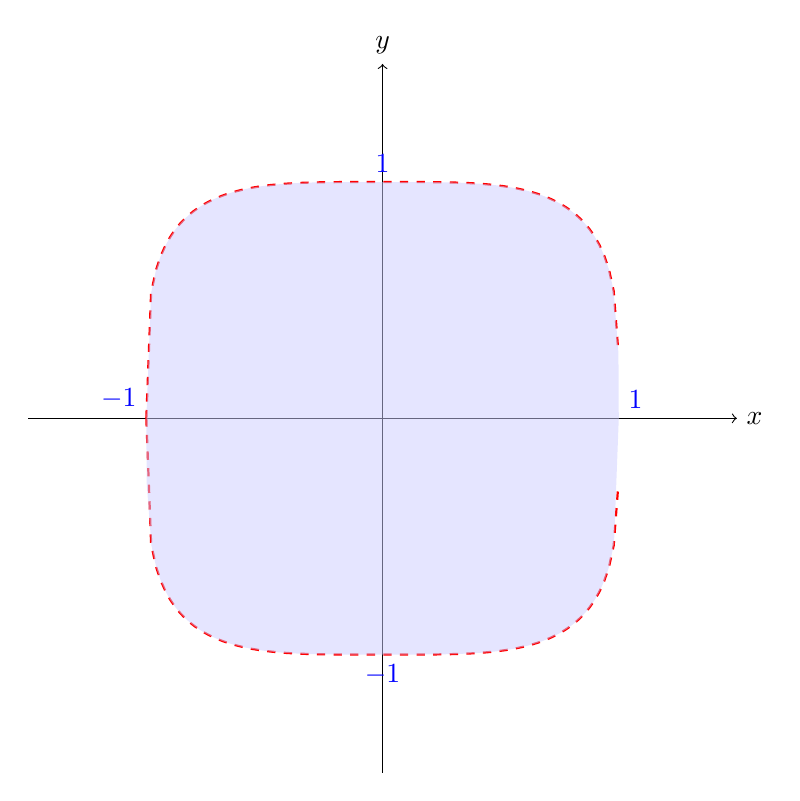
\begin{tikzpicture}[scale=3]
    %axis
    \draw[->] (-1.5,0) -- (1.5,0) node[right] {$x$};
    \draw[->] (0,-1.5) -- (0,1.5) node[above] {$y$};

    %boundry (dashes)
    \draw[thick, dashed, red] plot[domain=-1:1,samples=100] (\x, { (1 - abs(\x)^4)^(1/4) });
    \draw[thick, dashed, red] plot[domain=-1:1,samples=100] (\x, { -(1 - abs(\x)^4)^(1/4) });
    \fill[blue!20,opacity=0.5] plot[domain=-1:1,samples=100] (\x, { (1 - abs(\x)^4)^(1/4) }) -- plot[domain=1:-1,samples=100] (\x, { -(1 - abs(\x)^4)^(1/4) }) -- cycle;

    %labels
    \node[blue, above right] at (1,0) {$1$};
    \node[blue, above left] at (-1,0) {$-1$};
    \node[blue, above] at (0,1) {$1$};
    \node[blue, below] at (0,-1) {$-1$};
\end{tikzpicture}

The closed ball on metric
\[ d((a_{1},a_{2}),(b_{1},b_{2])) = (|b_{1} - a_{1}|^{4}  + |b_{2} - a_{2}|^4)^{\frac{1}{4}} \] is given by
\begin{align*}
B_{d}[(0,0),1] &= \{ (x,y) \in \R^{2} : d((x,y),(0,0)) \leq 1 \} \\[8pt]
&= \{ (x,y) \in \R^{2} : (|x - 0|^{4} + |y - 0|^{4})^{\frac{1}{4}} \leq 1 \} \\[8pt]
&= \{ (x,y) \in \R^{2} : (|x|^{4} + |y|^{4})^{\frac{1}{4}} \leq 1 \}      
\end{align*}    

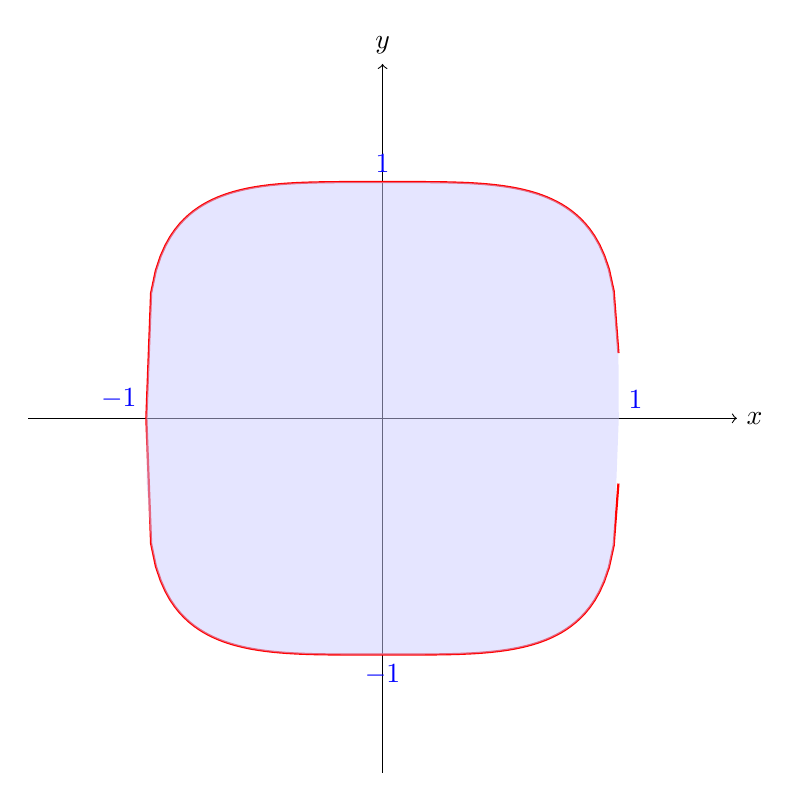
\begin{tikzpicture}[scale=3]
    %axis
    \draw[->] (-1.5,0) -- (1.5,0) node[right] {$x$};
    \draw[->] (0,-1.5) -- (0,1.5) node[above] {$y$};

    %boundry (solid)
    \draw[thick, red] plot[domain=-1:1,samples=100] (\x, { (1 - abs(\x)^4)^(1/4) });
    \draw[thick, red] plot[domain=-1:1,samples=100] (\x, { -(1 - abs(\x)^4)^(1/4) });
    \fill[blue!20,opacity=0.5] plot[domain=-1:1,samples=100] (\x, { (1 - abs(\x)^4)^(1/4) }) -- plot[domain=1:-1,samples=100] (\x, { -(1 - abs(\x)^4)^(1/4) }) -- cycle;

    %labels
    \node[blue, above right] at (1,0) {$1$};
    \node[blue, above left] at (-1,0) {$-1$};
    \node[blue, above] at (0,1) {$1$};
    \node[blue, below] at (0,-1) {$-1$};
\end{tikzpicture}

The sphere on metric
\[ d((a_{1},a_{2}),(b_{1},b_{2])) = (|b_{1} - a_{1}|^{4}  + |b_{2} - a_{2}|^4)^{\frac{1}{4}} \] is given by
\begin{align*}
S_{s}((0,0),1) &= \{ (x,y) \in \R^{2} : d((x,y),(0,0)) = 1 \} \\[8pt]
&= \{ (x,y) \in \R^{2} : (|x - 0|^{4} + |y - 0|^{4})^{\frac{1}{4}} = 1 \} \\[8pt]       
&= \{ (x,y) \in \R^{2} : (|x|^{4} + |y|^{4})^{\frac{1}{4}} = 1 \}
\end{align*}        

\begin{tikzpicture}[scale=3]
    %axis
    \draw[->] (-1.5,0) -- (1.5,0) node[right] {$x$};
    \draw[->] (0,-1.5) -- (0,1.5) node[above] {$y$};

    %boundry (solid)
    \draw[thick, red] plot[domain=-1:1,samples=100] (\x, { (1 - abs(\x)^4)^(1/4) });
    \draw[thick, red] plot[domain=-1:1,samples=100] (\x, { -(1 - abs(\x)^4)^(1/4) });

    %labels
    \node[blue, above right] at (1,0) {$1$};
    \node[blue, above left] at (-1,0) {$-1$};
    \node[blue, above] at (0,1) {$1$};
    \node[blue, below] at (0,-1) {$-1$};
\end{tikzpicture}

\qpart

The open ball on metric
\[ d((a_{1},a_{2}),(b_{1},b_{2})) = d_{0}(a_{1},b_{1}) + 6|b_{2} - a_{2}| \]

is given by
\begin{align*}
S_{s}((0,0),1) &= \{ (x,y) \in \R^{2} : d((x,y),(0,0)) < 1 \} \\[8pt]
&= \{ (x,y) \in \R^{2} : d_{0}(x,0) + 6|y - 0| < 1 \} \\[8pt]
&= \{ (x,y) \in \R^{2} : d_{0}(x,0) + 6|y| < 1 \}   
\end{align*}

\begin{tikzpicture}[scale=3]
    %axis
    \draw[->] (-0.5,0) -- (0.5,0) node[right] {$x$};
    \draw[->] (0,-1) -- (0,1) node[above] {$y$};

    %boundry (solid)
    \draw[dashed, thick, red] (0,-1/6) -- (0,1/6);
    
    %labels
    \node[blue, right] at (0,1/6) {$\frac{1}{6}$};
    \node[blue, right] at (0,-1/6) {$\frac{-1}{6}$};
  
\end{tikzpicture}

The closed ball on metric
\[ d((a_{1},a_{2}),(b_{1},b_{2])) = d_{0}(a_{1},b_{1}) + 6|b_{2} - a_{2}| \] is given by
\begin{align*}
B_{d}[(0,0),1] &= \{ (x,y) \in \R^{2} : d((x,y),(0,0)) \leq 1 \} \\[8pt]
&= \{ (x,y) \in \R^{2} : d_{0}(x,0) + 6|y - 0| \leq 1 \} \\[8pt]
&= \{ (x,y) \in \R^{2} : d_{0}(x,0) + 6|y| \leq 1 \}   
\end{align*}    

\begin{tikzpicture}[scale=3]
    %axis
    \draw[->] (-0.5,0) -- (0.5,0) node[right] {$x$};
    \draw[->] (0,-1) -- (0,1) node[above] {$y$};

    %boundry (solid)
    \draw[thick, red] (0,-1/6) -- (0,1/6);
    \fill[blue!20,opacity=0.5] (0,-1/6) -- (0,1/6) -- cycle;
    
    %labels
    \node[blue, right] at (0,1/6) {$\frac{1}{6}$};
    \node[blue, right] at (0,-1/6) {$\frac{-1}{6}$};

\end{tikzpicture}

The sphere on metric
\[ d((a_{1},a_{2}),(b_{1},b_{2])) = d_{0}(a_{1},b_{1}) + 6|b_{2} - a_{2}| \] is given by
\begin{align*}
S_{s}((0,0),1) &= \{ (x,y) \in \R^{2} : d((x,y),(0,0)) = 1 \} \\[8pt]
&= \{ (x,y) \in \R^{2} : d_{0}(x,0) + 6|y - 0| = 1 \} \\[8pt]
&= \{ (x,y) \in \R^{2} : d_{0}(x,0) + 6|y| = 1 \}   
\end{align*}

\begin{tikzpicture}[scale=3]
    %axis
    \draw[->] (-0.5,0) -- (0.5,0) node[right] {$x$};
    \draw[->] (0,-1) -- (0,1) node[above] {$y$};

    %boundry (solid)
    \draw[thick, red] (0,-1/6) -- (0,1/6);
    
    %labels
    \node[blue, right] at (0,1/6) {$\frac{1}{6}$};
    \node[blue, right] at (0,-1/6) {$\frac{-1}{6}$};
\end{tikzpicture}



\end{question}

\end{document}